% To je predloga za poročila o domačih nalogah pri predmetih, katerih
% nosilec je Blaž Zupan. Seveda lahko tudi dodaš kakšen nov, zanimiv
% in uporaben element, ki ga v tej predlogi (še) ni. Več o LaTeX-u izveš na
% spletu, na primer na http://tobi.oetiker.ch/lshort/lshort.pdf.
%
% To predlogo lahko spremeniš v PDF dokument s pomočjo programa
% pdflatex, ki je del standardne instalacije LaTeX programov.

\documentclass[a4paper,11pt]{article}
\usepackage{csquotes}
\usepackage{a4wide}
\usepackage{fullpage}
\usepackage[utf8x]{inputenc}
\usepackage[slovene]{babel}
\selectlanguage{slovene}
\usepackage[toc,page]{appendix}
\usepackage[pdftex]{graphicx} % za slike
\usepackage{setspace}
\usepackage{color}
\definecolor{light-gray}{gray}{0.95}
\usepackage{listings} % za vključevanje kode
\usepackage{hyperref}
\renewcommand{\baselinestretch}{1.2} % za boljšo berljivost večji razmak
\renewcommand{\appendixpagename}{Priloge}

\lstset{ % nastavitve za izpis kode, sem lahko tudi kaj dodaš/spremeniš
language=Python,
basicstyle=\footnotesize,
basicstyle=\ttfamily\footnotesize\setstretch{1},
backgroundcolor=\color{light-gray},
}

\title{Podobnost jezikov}
\author{Tilen Venko (63140280)}
\date{\today}

\begin{document}

\maketitle

\section{Uvod}

Prvi cilj naloge je bil, da zgradimo hierarhijo vsaj dvajsetih jezikov, ki vsebujejo vsaj 2 tuji pisavi in jo komentiramo. Drugi cilj pa je, da na podlagi besedil, ki smo jih obdelovali znamo iz poljubnega besedila v enem od teh jezikov ugotoviti, v kakšnem jeziku je to besedilo in podati, s kakšno verjetnostjo lahko to trdimo.

\section{Podatki}

Jezike smo pridobili iz spletne strani združenih narodov iz Splošne deklaracije človekovih pravic. Tako je besedilo, ki ga preverjami enako v vseh jezikih, kar naj bo dalo boljše rezultate pri gradnji hierarhije jezikov. Besedila se nahajajo v datoteki \path{/human_rights/ready/}. Za svojo nalogo sem si izbral 22 evropskih jezikov:
\begin{itemize}
	\item angleščina
	\item beloruščina
	\item bosanščina v cirilici in latinici 
	\item češčina 
	\item danščina
	\item finščina
	\item francoščina
	\item grščina v grški pisavi
	\item italijanščina
	\item latinščina
	\item madžarščina
	\item makedonščina
	\item nizozemščina
	\item nemščina
	\item norveščina
	\item polščina
	\item portugalščina
	\item ruščina
	\item slovaščina
	\item slovenščina
	\item srbščina v cirilici in latinici
	\item španščina
\end{itemize}


Besedila nad katerimi sem preverjal ali program pravilno zazna jezik besedila se nahajajo v mapi \path{\test}. Besedila sem generiral s spletnim orodjem \url{http://randomtextgenerator.com/}. Tam sem generiral besedila v angleščini, francoščini, nemščini, grščini v grški pisavi, italijanščini, srbščini v cirilici. S portala MMC rtvslo \url{https://www.rtvslo.si/slovenija/anja-kopac-mrak-cerar-ni-zahteval-mojega-odstopa/406291} pa sem pridobil članek v slovenščini.

\section{Metode}

Iz besedil sem najprej poskušal odstranit nepotrebne podatke. Tako sem vse črke spremenil v male, odstranil prehode v novo vrstico in jih nadomestil s presledki. Besedilo sem tudi dekodiral iz unikode, zato da so vsa besedila v enaki pisavi, latinici. Brez tega bi si namreč bosanščina v latinici in cirilici ne bili nič podobni, prav tako pa ne bi mogel grščine primerjati z ostalimi jeziki. \\
Besedilo sem nato razbil na terke črk, ki so privzeto velikosti 3, in preštel kolikokrat se kakšna terka pojavi. Nad matriko teh terk sem nato klical funkcijo linkage, ki je za parameter "matric", prejela mojo funkcijo cosinus, v kateri sem implementiral metodo za izračun kosinusne razdalje.\\
Nad podatki, ki sem jih dobil iz funkcije linkage sem nato klical še funkcijo dendrogram in izrisal dendrogram hierarhije jezikov.
\\
\\
Drugega dela naloge, kjer sem moral implementirati metodo, s katero sem ugotavljal v kakšnem jeziku je podano besedilo, sem se lotil na zelo podoben način, da sem najprej očistil besedilo enako, kot prej. Nato pa sem za vse jezike od prej in podanim besedilom izračunal kosinusno razdaljo med njimi izmed teh izbral tri z najmanjšo razdaljo in jih vrnil, kot tri najbolj verjetne jezike, v katerem je to besedilo, za najbolj verjeten jezik pa sem podal tudi verjetnost, da je iskano besedilo v tem jeziku.


\section{Rezultati}
\subsection{Hierarhija jezikov}


\begin{center}
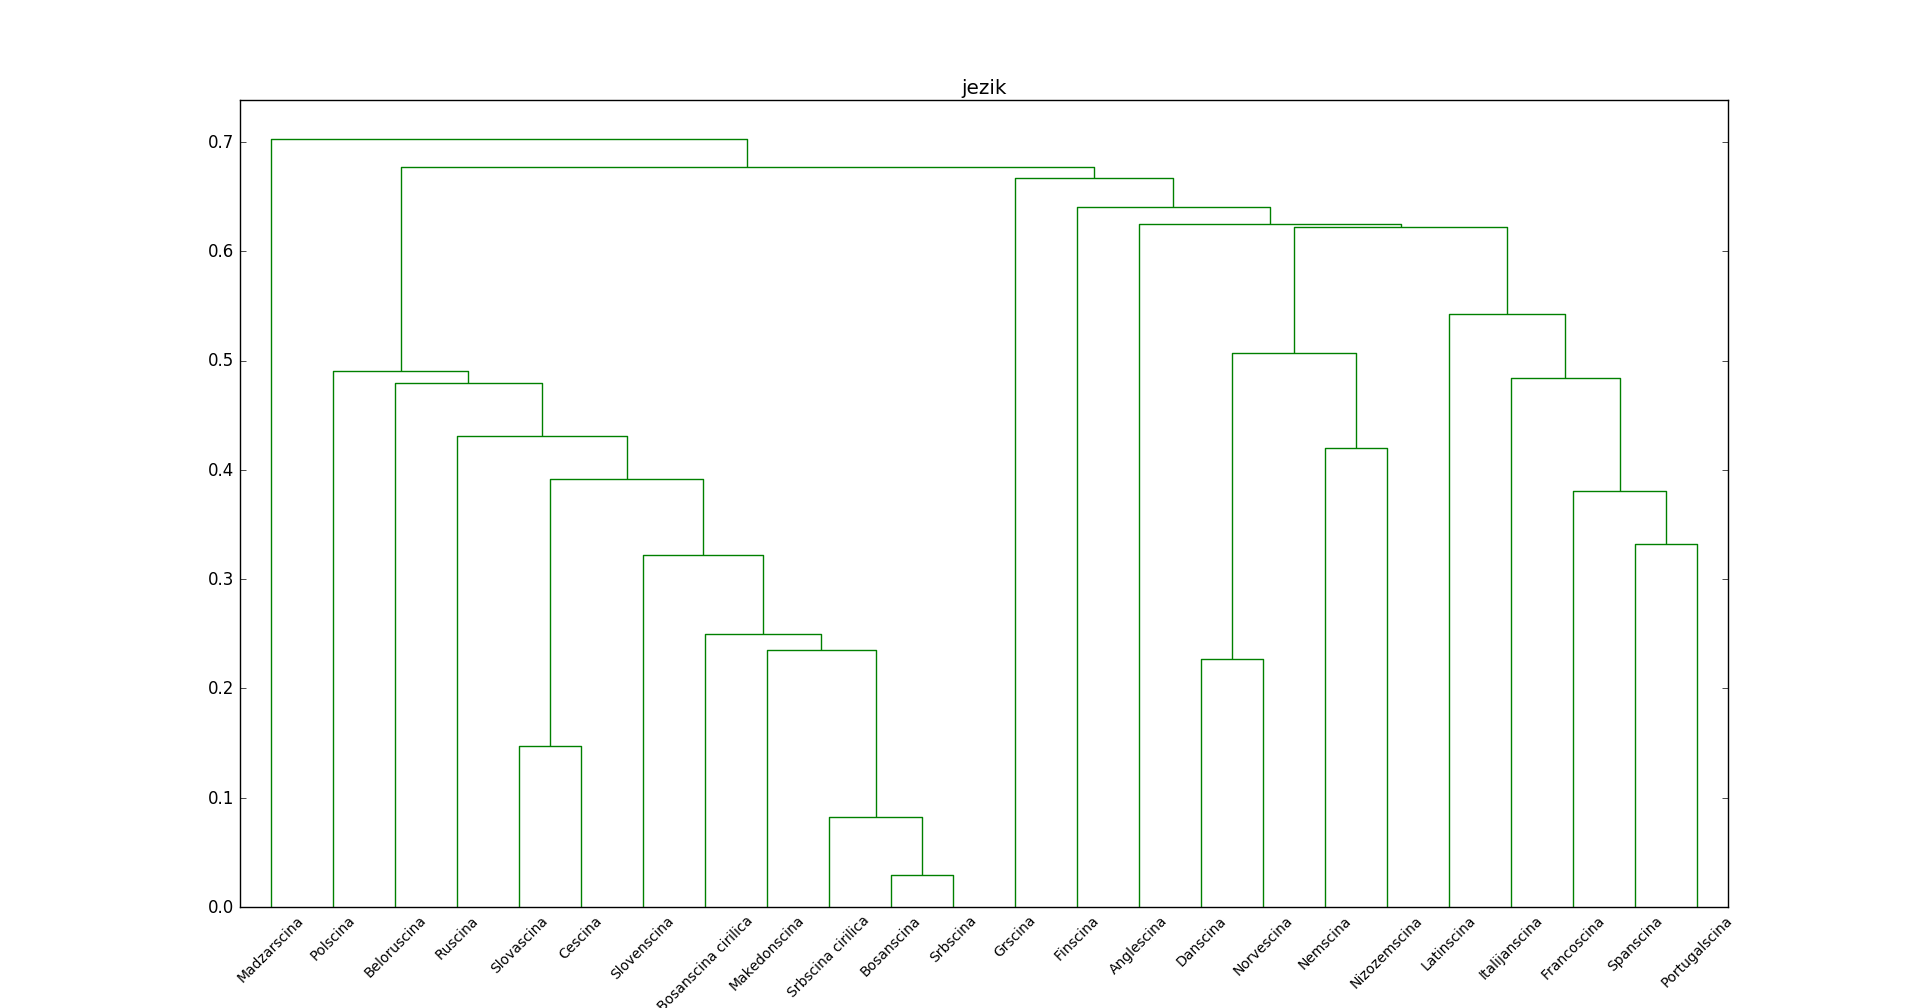
\includegraphics[scale=0.3]{dendrogram.png}
\caption{Dendrogram hierarhije jezikov}
\label{slika1}
\end{center}


Podatki v dendrogramu so takšni, kot bi jih pričakovali. slovanski jeziki so blizu skupaj pri čemer lahko ločimo vzhodnoslovanske jezike (slovaščina in češčina) in jugoslovanske jezike, pri čemer pa je polščina izjema. Srbščina in bosanščina v cirilici in latinici nista čisto skupaj zato, ker ko dekodiramo iz unikode, se določeni znaki zapisejo malo drugače, kot pa so zapisano v latinici. Vidimo lahko tudi skupino romanskih in pa germanskih jezikov, ki pa nista tako očitno ločeni med sabo, kot sta od slovanske jezikovne skupine. Opazimo pa lahko tudi, da grščina, finščina in madžarščina ne spadajo v nobeno od teh jezikovnih skupin, pri čemer najbolj izstopa madžarščina.

\subsection{Prepoznava jezika iz besedila}
Če programu podam generirano besedilo v angleščini mi vrne:\\

\begin{displayquote}
Besedilo je v jeziku Angleščina z verjetnostjo 38.426\% lahko pa je tudi v jezikih Francoščina ali Danščina.
\end{displayquote}

Program nam zna dobro povedati v kakšnem jeziku je besedilo, vendar to lahko trdi z manjšo gotovostjo.

\section{Izjava o izdelavi domače naloge}
Domačo nalogo in pripadajoče programe sem izdelal sam.



\end{document}
